
\documentclass[10pt]{beamer}
\usetheme{umbc2}
\useinnertheme{umbcboxes}
\setbeamercolor{umbcboxes}{bg=violet!12,fg=black}

\usepackage{longtable}
\usepackage{tabu}

\newcommand{\ul}{\underline}
\newcommand{\be}{\begin{equation}}
\newcommand{\ee}{\end{equation}}
\newcommand{\bdm}{\begin{displaymath}}
\newcommand{\edm}{\end{displaymath}}
\newcommand{\bea}{\begin{eqnarray}}
\newcommand{\eea}{\end{eqnarray}}
\newcommand{\bsea}{\begin{subeqnarray}}
\newcommand{\esea}{\end{subeqnarray}}
\newcommand{\mb}[1]{\mbox{#1}}
\newcommand{\mc}[3]{\multicolumn{#1}{#2}{#3}}
\newcommand{\bm}[1]{\mbox{\bf #1}}
\newcommand{\bmm}[1]{\mbox{\boldmath$#1$\unboldmath}}
\newcommand{\bmell}{\bmm\ell}
\newcommand{\hateps}{\widehat{\bmm\varepsilon}}
\newcommand{\graybox}[1]{\psboxit{box .9 setgray fill}{\fbox{#1}}}
\newcommand{\mdeg}[1]{\mbox{$#1^{\mbox{\scriptsize o}}$}}
\newcommand{\dd}{\mbox{\footnotesize{$\nabla \! \Delta$}}}
\newcommand{\p}{\partial\,}
\renewcommand{\d}{\mbox{d}}
\newcommand{\dspfrac}{\displaystyle\frac}
\newcommand{\nl}{\\[4mm]}

\title{Processing GNSS Data in Real-Time}

\author{Leo\v{s} Mervart}

\institute{TU Prague}

\date{Frankfurt, January 2014}

% \AtBeginSection[]
% {
%   \begin{frame}
%     \frametitle{Table of Contents}
%     \tableofcontents[currentsection]
%   \end{frame}
% }

\begin{document}

%%%%%%%%%%%%%%%%%%%%%%%%%%%%%%%%%%%%%%%%%%%%%%%%%%%%%%%%%%%%%%%%%%%%%%%%%%%%%%%%

\begin{frame}
  \titlepage
\end{frame}

%%%%%%%%%%%%%%%%%%%%%%%%%%%%%%%%%%%%%%%%%%%%%%%%%%%%%%%%%%%%%%%%%%%%%%%%%%%%%%%%

\begin{frame}
\frametitle{Medieval Times of GNSS (personal memories)}

\begin{description}
\item[1991] Prof. Gerhard Beutler became the director of the Astronomical Institute, University of
  Berne. The so-called Bernese GPS Software started to be used for (post-processing) analyzes of
  GNSS data.
\item[1992] LM started his PhD study at AIUB.
\item[1992] Center for Orbit Determination in Europe (consortium of AIUB, Swisstopo, BKG, IGN, and
  IAPG/TUM) established. Roughly at that time LM met Dr. Georg Weber for the first time.
\item[1993] International GPS Service formally recognized by the IAG.
\item[1994] IGS began providing GPS orbits and other products routinely (January, 1).
\item[1995] GPS declared fully operational.
\end{description}

\end{frame}

%%%%%%%%%%%%%%%%%%%%%%%%%%%%%%%%%%%%%%%%%%%%%%%%%%%%%%%%%%%%%%%%%%%%%%%%%%%%%%%%

\begin{frame}
\frametitle{CODE-Related Works in 1990's}

\begin{itemize}
\item The Bernese GPS Software was the primary tool for CODE analyzes (Fortran~77).
\item IGS reference network was sparse.
\item Real-time data transmission limited (Internet was still young, TCP/IP widely accepted 1989).
\item CPU power of then computers was limited (VAX/VMS OS used at AIUB).
\end{itemize}

In 1990's high precision GPS analyzes were almost exclusively performed in post-processing mode.
The typical precise application of GPS at that time was the processing of a network of static
GPS-only receivers for the estimation of station coordinates.

\end{frame}

%%%%%%%%%%%%%%%%%%%%%%%%%%%%%%%%%%%%%%%%%%%%%%%%%%%%%%%%%%%%%%%%%%%%%%%%%%%%%%%%

\begin{frame}
\frametitle{Tempora mutantur (and maybe ``nos mutamur in illis'')}

\begin{center}
  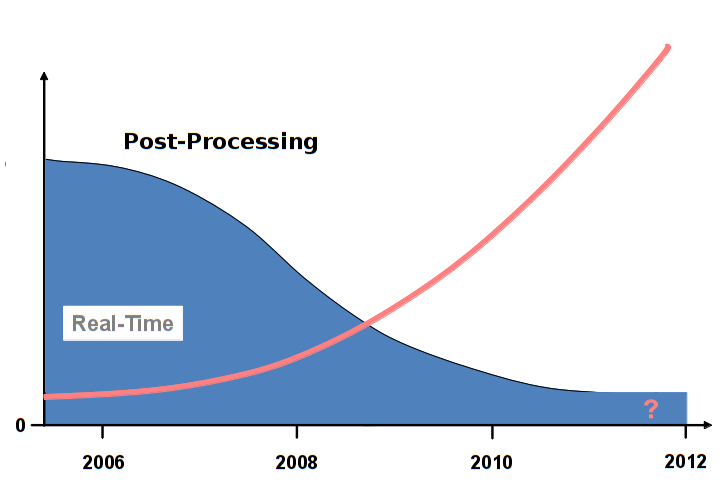
\includegraphics[width=0.7\textwidth,angle=0]{pp_vs_rt.png}
\end{center}

\end{frame}


%%%%%%%%%%%%%%%%%%%%%%%%%%%%%%%%%%%%%%%%%%%%%%%%%%%%%%%%%%%%%%%%%%%%%%%%%%%%%%%%

\begin{frame}
\frametitle{}

\end{frame}

%%%%%%%%%%%%%%%%%%%%%%%%%%%%%%%%%%%%%%%%%%%%%%%%%%%%%%%%%%%%%%%%%%%%%%%%%%%%%%%%

\begin{frame}
\frametitle{}

\end{frame}

%%%%%%%%%%%%%%%%%%%%%%%%%%%%%%%%%%%%%%%%%%%%%%%%%%%%%%%%%%%%%%%%%%%%%%%%%%%%%%%%

\begin{frame}
\frametitle{}

\end{frame}

\end{document}
